%!TEX root = ../report_template.tex
\section*{Methods}
%Todo: Think about citations



\textbf{The Pearson correlation coefficient}, denoted as $r_{X,Y}$, is a statistical measure used to assess the linear relationship between two sets of data, $X$ and $Y$. It is computed as the ratio of the sample covariance of the $X$ and $Y$ to the product of their sample standard deviations: %Todo: Source
\begin{equation}
    r_{X,Y} = \frac{\sum_{i=1}^n (X_i - \overline{X}) (Y_i - \overline{Y})}{\sqrt{\sum_{i=1}^n(X_i-\overline{X})^2 \cdot \sum_{i=1}^n(Y_i-\overline{Y})^2}}
\end{equation}


\paragraph{Datasets:}
The basis for the analysis of the German school system are the average final Abitur grades. The grades are published every year by the \citeauthor{kultusminister_konferenz_abiturnoten_nodate}. Each file contains the count of children per written grade and federal state. The grades are defined in $0.1$ steps, with $4.0$ as the worst and $1.0$ as the best grade. Furthermore, the amount of children who failed with a grade worse than $4.0$ is aggregated in an additional column.

The second dataset is provided in the \textit{Fachreport Schuljahr 2020/21} of the \citeauthor{statistische_bundesamt_allgemeinbildende_2022} and contains the number of teachers from 1992 until 2020. The dataset groups them primarily according to their contract type, federal state, and school type. This paper merges the teacher counts with two student datasets, which are published in the \textit{Genesis} database of the \citeauthor{statistische_bundesamt_statistisches_2023}. Both provide the number of students as different groupings and aggregations. The first contains the number of children per grade and school type  for the years 1998 to 2022. In contrast, the second table provides the absolute amount of children, leavers, and beginners in each federal state from 1997 to 2022. Therefore, the analysis of the merged dataset can only be conducted separately for school types and federal states.

The dataset \textit{Repeaters}, derived from the \textit{GENESIS} Database of the \citeauthor{statistische_bundesamt_statistisches_2023}, encompasses data spanning from the academic year 1998/99 through 2022/23.  It includes data on the number of repeaters categorized by federal state, year, school type, grade, and gender. 

\paragraph{Figures}
%TODO: Better beginning
\autoref{fig:heatmap_correlation_students_per_teacher_repeaters_budget} presents a visualization of the Pearson correlation coefficients, analyzing the relationship between the number of students per teacher and the average number of repeaters, as well as the educational budget per state. 

Initially, to compute the average number of repeaters, the \textit{Number of Repeaters}dataset is aggregated by \textit{Federal States} and \textit{Years}, with the mean value being calculated for each grouping. Subsequently, all datasets were merged, using \textit{Federal States} and \textit{Years} as the common attributes for alignment. 

Finally, for each state, the Pearson correlation coefficient was calculated across different years to ascertain the correlation between students per teacher and the budget, as well as the average amount of repeaters.

In order to visualize the data over the states a heatmap for the german federal states is created. Therefor the Pearson correlation coefficients are normalized to the used colormap scale. Each state receives the appropriate computed color then.

\begin{figure}[h]
    \centering
    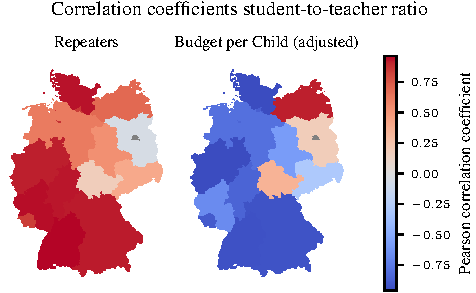
\includegraphics{fig/fig_heatmap_correlation_students_per_teacher_repeaters_budget.pdf}
    \caption{Pearson correlation coefficients between students per teacher and budget, such as repeaters.}
    \label{fig:heatmap_correlation_students_per_teacher_repeaters_budget}
\end{figure}
